\documentclass[12pt, a4paper, simple]{eskdtext}

\usepackage{hyperref}
\usepackage{_env/gpi_global.env}
\usepackage{_env/gpi_report.env}
\usepackage{_sty/gpi_lst}
\usepackage{_sty/gpi_toc}
\usepackage{_sty/gpi_t}
\usepackage{_sty/gpi_p}
\usepackage{_sty/gpi_u}

% Код
% \ESKDletter{О}{Л}{Р}
% \def \gpiDocTypeNum {81}
% \def \gpiDocVer {00}
% \def \gpiCode {\ESKDtheLetterI\ESKDtheLetterII\ESKDtheLetterIII.\gpiStudentGroupName\gpiStudentGroupNum.\gpiStudentCard-0\gpiDocNum~\gpiDocTypeNum~\gpiDocVer}

\def \gpiDocTopic {Отчёт лабораторной работы №\gpiDocNum}

% Графа 1 (наименование изделия/документа)
% \ESKDcolumnI {\ESKDfontII \gpiTopic \\ \gpiDocTopic}

% Графа 2 (обозначение документа)
% \ESKDsignature {\gpiCode}

% Графа 9 (наименование или различительный индекс предприятия) задает команда
% \ESKDcolumnIX {\gpiDepartment}

% Графа 11 (фамилии лиц, подписывающих документ) задают команды
% \ESKDcolumnXIfI {\gpiStudentSurname}
% \ESKDcolumnXIfII {\gpiTeacherSurname}
% \ESKDcolumnXIfV {\gpiTeacherSurname}

\begin{document}
    \begin{ESKDtitlePage}
    \ESKDstyle{empty}
    \begin{center}
        \gpiMinEdu \\
        \gpiEdu \\
        \gpiKaf \\
    \end{center}

    \vfill

    \begin{center}
        \gpiTopic
    \end{center}

    \vfill

    \begin{center}
        \textbf{\gpiDocTopic} \\
        ПО ДИСЦИПЛИНЕ \gpiDiscipline \\
    \end{center}

    \vfill

    \begin{flushright}
        \begin{minipage}[t]{7cm}
            Выполнил:\\
            \PageTitleStudentInfo
            \PageTitleDateField
            \hspace{0pt}

            Проверил:\\
            \PageTitleTeacherInfo
            \PageTitleDateField
        \end{minipage}
    \end{flushright}

    \vfill

    \begin{center}
        \PageTitleCity~\ESKDtheYear
    \end{center}
\end{ESKDtitlePage}

    \ESKDstyle{empty}
    \begin{center}
        \textbf{\gpiDocTopic}
    \end{center}

    % = = = = = = = =
    \paragraph{} \textbf{Тема}: <<\gpiTopicRep>>

    \paragraph{} \textbf{Цель}:
    освоить приемы тестирования кода на примере использования библиотеки JUnit.

    % \paragraph{} \textbf{Разработка дизайна}:

    % \begin{figure}[!h]
    %     \centering
    %     \includegraphics[]
    %         {_assets/ClassDiagram.png}
    %     \caption{Диграмма классов}
    % \end{figure}

    \paragraph{} \textbf{Что нужно сделать}:

    \textbf{Задание 1 – Введение в JUnit}

\begin{itemize}
    \item Создаете новый класс и скопируйте код класса Sum;
    \item Создаете тестовый класс SumTest;
    \item Напишите тест к методу Sum.accum и проверьте его исполнение.
    Тест должен проверять работоспособность функции accum.
    \item Очевидно, что если передать слишком большие значения в Sum.accum, то случится переполнение.
    Модифицируйте функцию Sum.accum, чтобы она возвращала значение типа long и напишите новый тест,
    проверяющий корректность работы функции с переполнением.
    Первый тест должен работать корректно.
\end{itemize}

    \begin{lstlisting}[language=java, name=Пример кода для задания 1]
public class Sum {
    public static int accum (int ... values) {
        int result = 0;
        for (int i = 0; i < values.length; i++) {
            result += values[i];
        }
        return result;
    }
}
\end{lstlisting}
    
    \paragraph{} \textbf{Исходный код}: 

    \lstinputlisting[language=java, name=src/main/java/com/example/Sum.java]
    {../sources/SPP_2sem_PO4_Galanin_lab5/src/main/java/com/example/Sum.java}

    \lstinputlisting[language=java, name=src/test/java/com/example/SumTest.java]
    {../sources/SPP_2sem_PO4_Galanin_lab5/src/test/java/com/example/SumTest.java}

    \begin{figure}[!h]
        \centering
        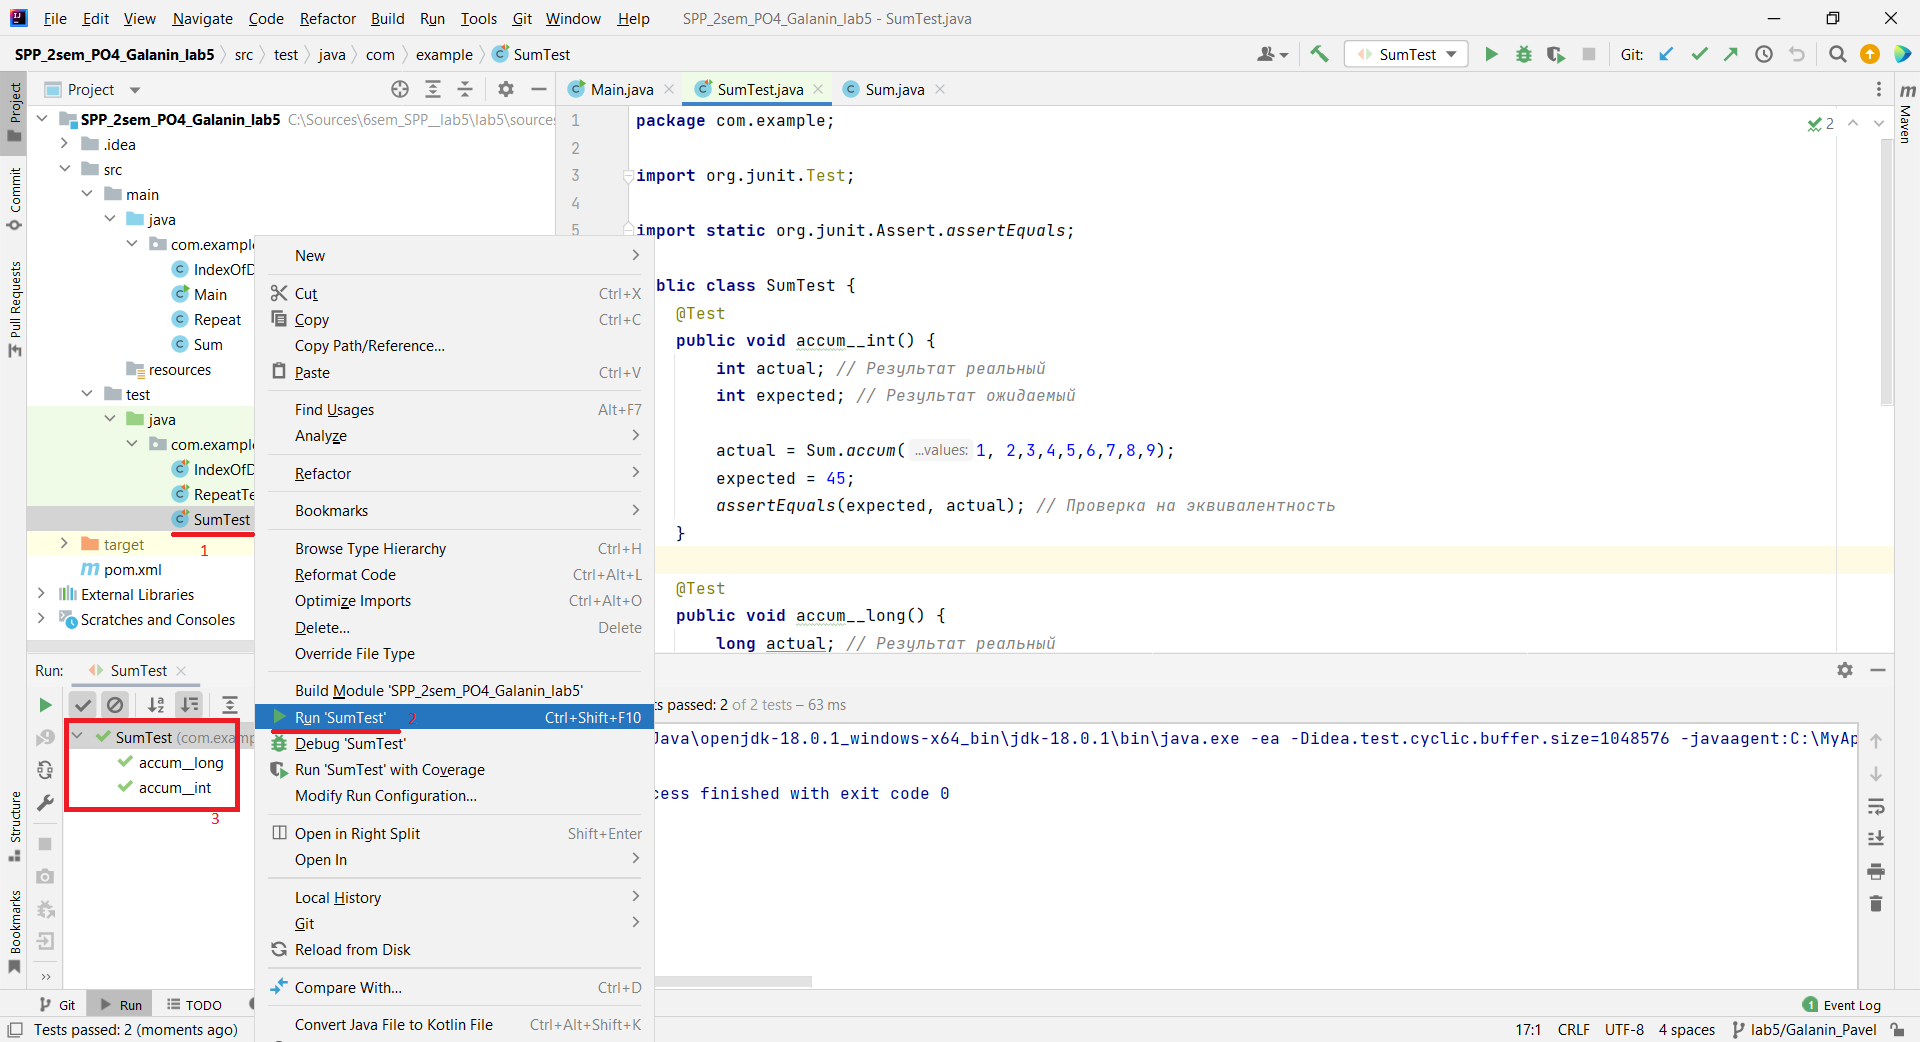
\includegraphics[width=16cm]
            {_assets/SumTest.png}
        \caption{Скриншот пройденных тестов класса Sum}
    \end{figure}

    \newpage

    \paragraph{} \textbf{Что нужно сделать}:

    \textbf{Задание 2 – Тестирование функций}

    Подготовка к выполнению:
  
    \begin{itemize}
        \item Создайте новый проект в рабочей IDE;
        \item Создайте класс StringUtils, в котором будут находится реализуемые функции;
        \item Напишите тесты для реализуемых функций.
    \end{itemize}

    Написать тесты к методу, а затем реализовать сам метод по заданной спецификации.
    
    Варианты:

    5) Реализуйте и протестируйте метод int indexOfDifference(String str1, String str2),
    который сравнивает две строки и возвращает индекс той позиции,
    в которой они различаются.
    Например, indexOfDifference("i am a machine" , "i am a robot") должно вернуть 7.

    Спецификация метода:

    \begin{lstlisting}[language=java, name=Пример кода для задания 2 (вариант 5)]
indexOfDifference(null, null) = NullPointerException
indexOfDifference("", "") = -1
indexOfDifference("", "abc") = 0
indexOfDifference("abc", "") = 0
indexOfDifference("abc", "abc") = -1
indexOfDifference("ab", "abxyz") = 2
indexOfDifference("abcde", "abxyz") = 2
indexOfDifference("abcde", "xyz") = 0
\end{lstlisting}
    
    \paragraph{} \textbf{Исходный код}: 

    \lstinputlisting[language=java, name=src/main/java/com/example/IndexOfDifference.java]
    {../sources/SPP_2sem_PO4_Galanin_lab5/src/main/java/com/example/IndexOfDifference.java}

    \lstinputlisting[language=java, name=src/test/java/com/example/IndexOfDifferenceTest.java]
    {../sources/SPP_2sem_PO4_Galanin_lab5/src/test/java/com/example/IndexOfDifferenceTest.java}

    \begin{figure}[!h]
        \centering
        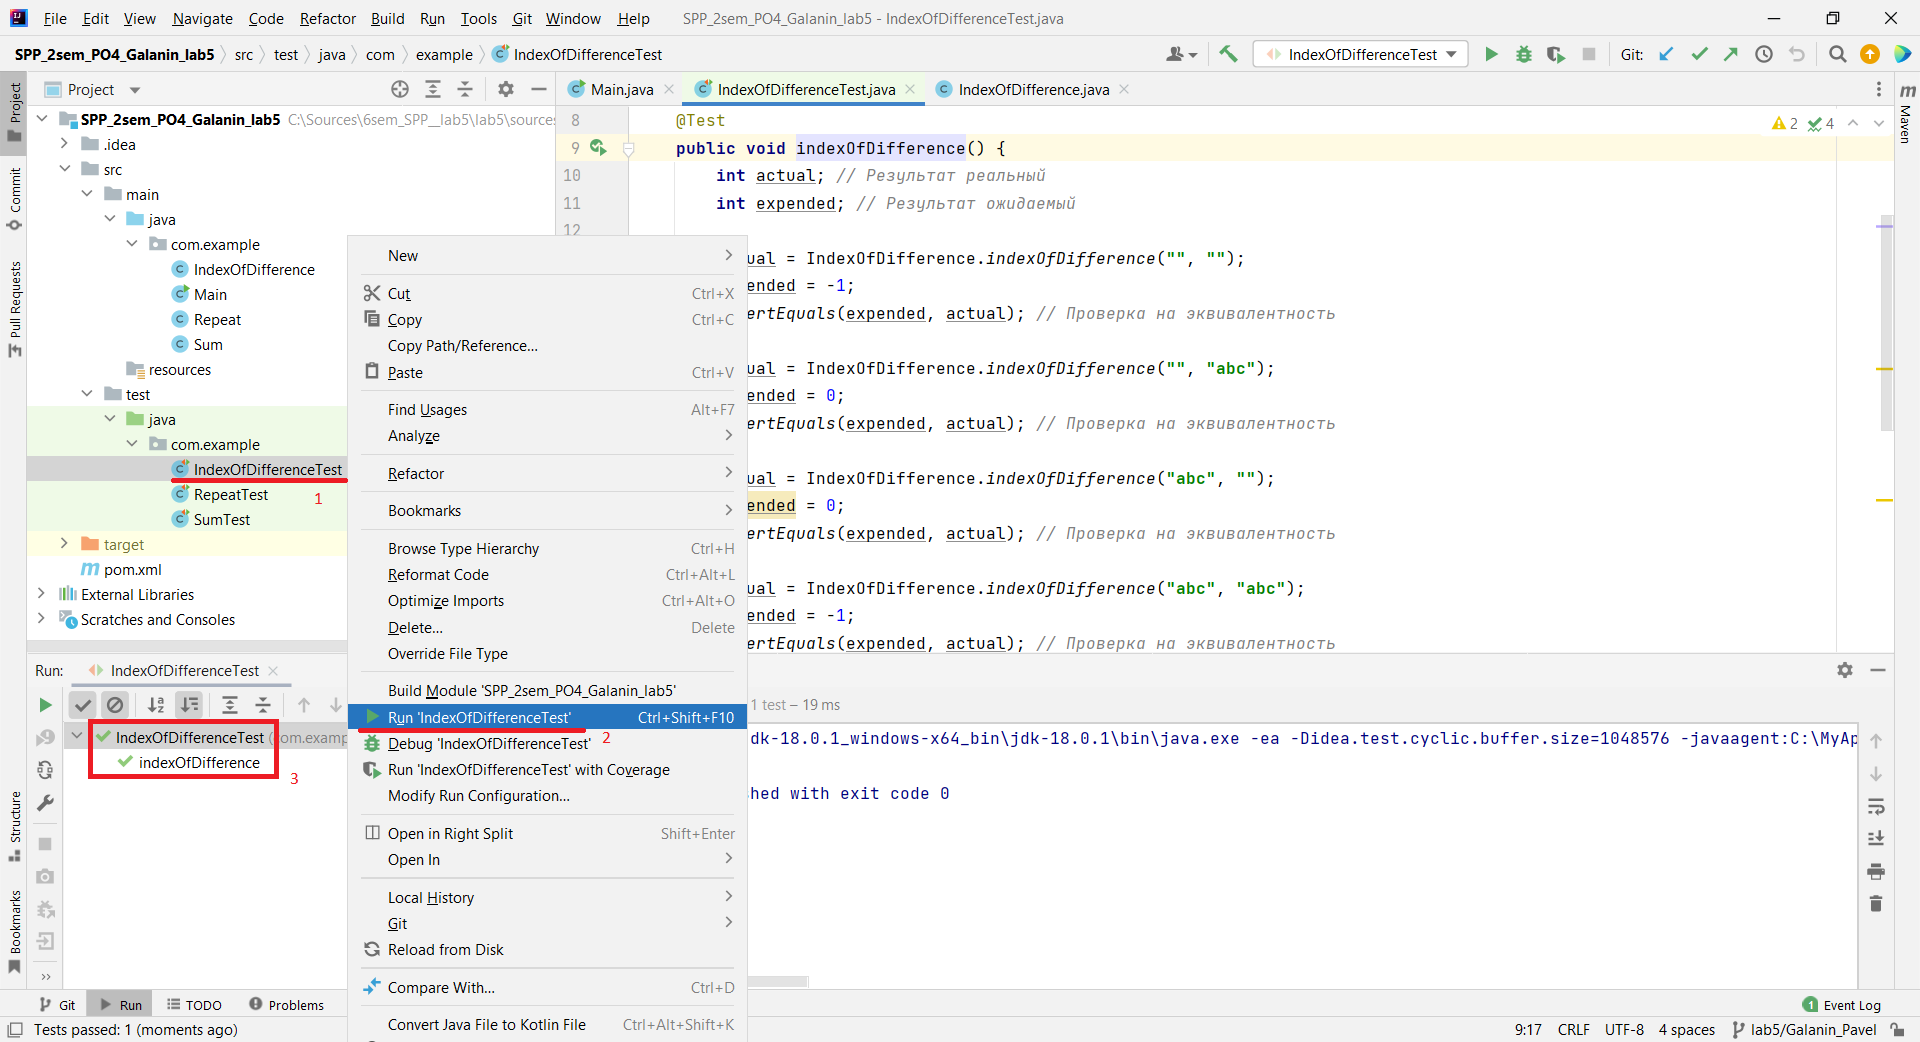
\includegraphics[width=16cm]
            {_assets/IndexOfDifferenceTest.png}
        \caption{Скриншот пройденных тестов класса IndexOfDifference}
    \end{figure}

    \newpage

    \paragraph{} \textbf{Что нужно сделать}:

    \textbf{Задание 3 – Поиск ошибок, отладка и тестирование классов}

    \begin{enumerate}
        \item[1)] Импорт проекта Импортируйте один из проектов по варианту:
        \item[-] Stack – проект содержит реализацию стека на основе связного списка: Stack.java.
        \item[-] Queue – содержит реализацию очереди на основе связного списка: Queue.java.
        Разберитесь как реализована ваша структура данных. Каждый проект содержит:
        \item[-] Клиент для работы со структурой данных и правильности ввода данных реализации (см. метод main()).
        \item[-] TODO-декларации, указывающие на нереализованные методы и функциональность.
        \item[-] FIXME-декларации, указывающую на необходимые исправления.
        \item[-] Ошибки компиляции (Синтаксические)
        \item[-] Баги в коде (!).
        \item[-] Метод check() для проверки целостности работы класса.
        
        \item[2)] Поиск ошибок
        \item[-] Исправить синтаксические ошибки в коде.
        \item[-] Разобраться в том, как работает код, подумать о том, как он должен работать и найти допущенные баги.
        
        \item[3)] Внутренняя корректность
        \item[-] Разобраться что такое утверждения (assertions) в коде и как они включаются в Java.
        \item[-] Заставить ваш класс работать вместе с включенным методом check.
        \item[-] Выполнить клиент (метод main() класса) передавая данные в структуру используя включенные проверки (assertions).
        
        \item[4)] Реализация функциональности
        \item[-] Реализовать пропущенные функции в классе.
        \item[-] См. документацию перед методом относительно того, что он должен делать и какие исключения выбрасывать. 
        \item[-] Добавить и реализовать функцию очистки состояния структуры данных.
        
        \item[5)] Написание тестов
        \item[-] Все функции вашего класса должны быть покрыты тестами.
        \item[-] Использовать фикстуры для инициализации начального состояния объекта.
        \item[-] Итого, должно быть несколько тестовых классов,
        в каждом из которых целевая структура данных создается в фикстуре в некотором инициализированном состоянии
        (пустая, заполненная и тд), а после очищается.
        \item[-] Написать тестовый набор, запускающий все тесты.
    \end{enumerate}

    \paragraph{} \textbf{Исходный код}: 

    \lstinputlisting[language=java, name=src/queue/QueueClient.java]
    {../sources/SPP_2sem_PO4_Galanin_lab5_Queue/src/queue/QueueClient.java}

    \lstinputlisting[language=java, name=src/queue/Queue.java]
    {../sources/SPP_2sem_PO4_Galanin_lab5_Queue/src/queue/Queue.java}

    \lstinputlisting[language=java, name=test/queue/QueueTest.java]
    {../sources/SPP_2sem_PO4_Galanin_lab5_Queue/test/queue/QueueTest.java}

    \begin{figure}[!h]
        \centering
        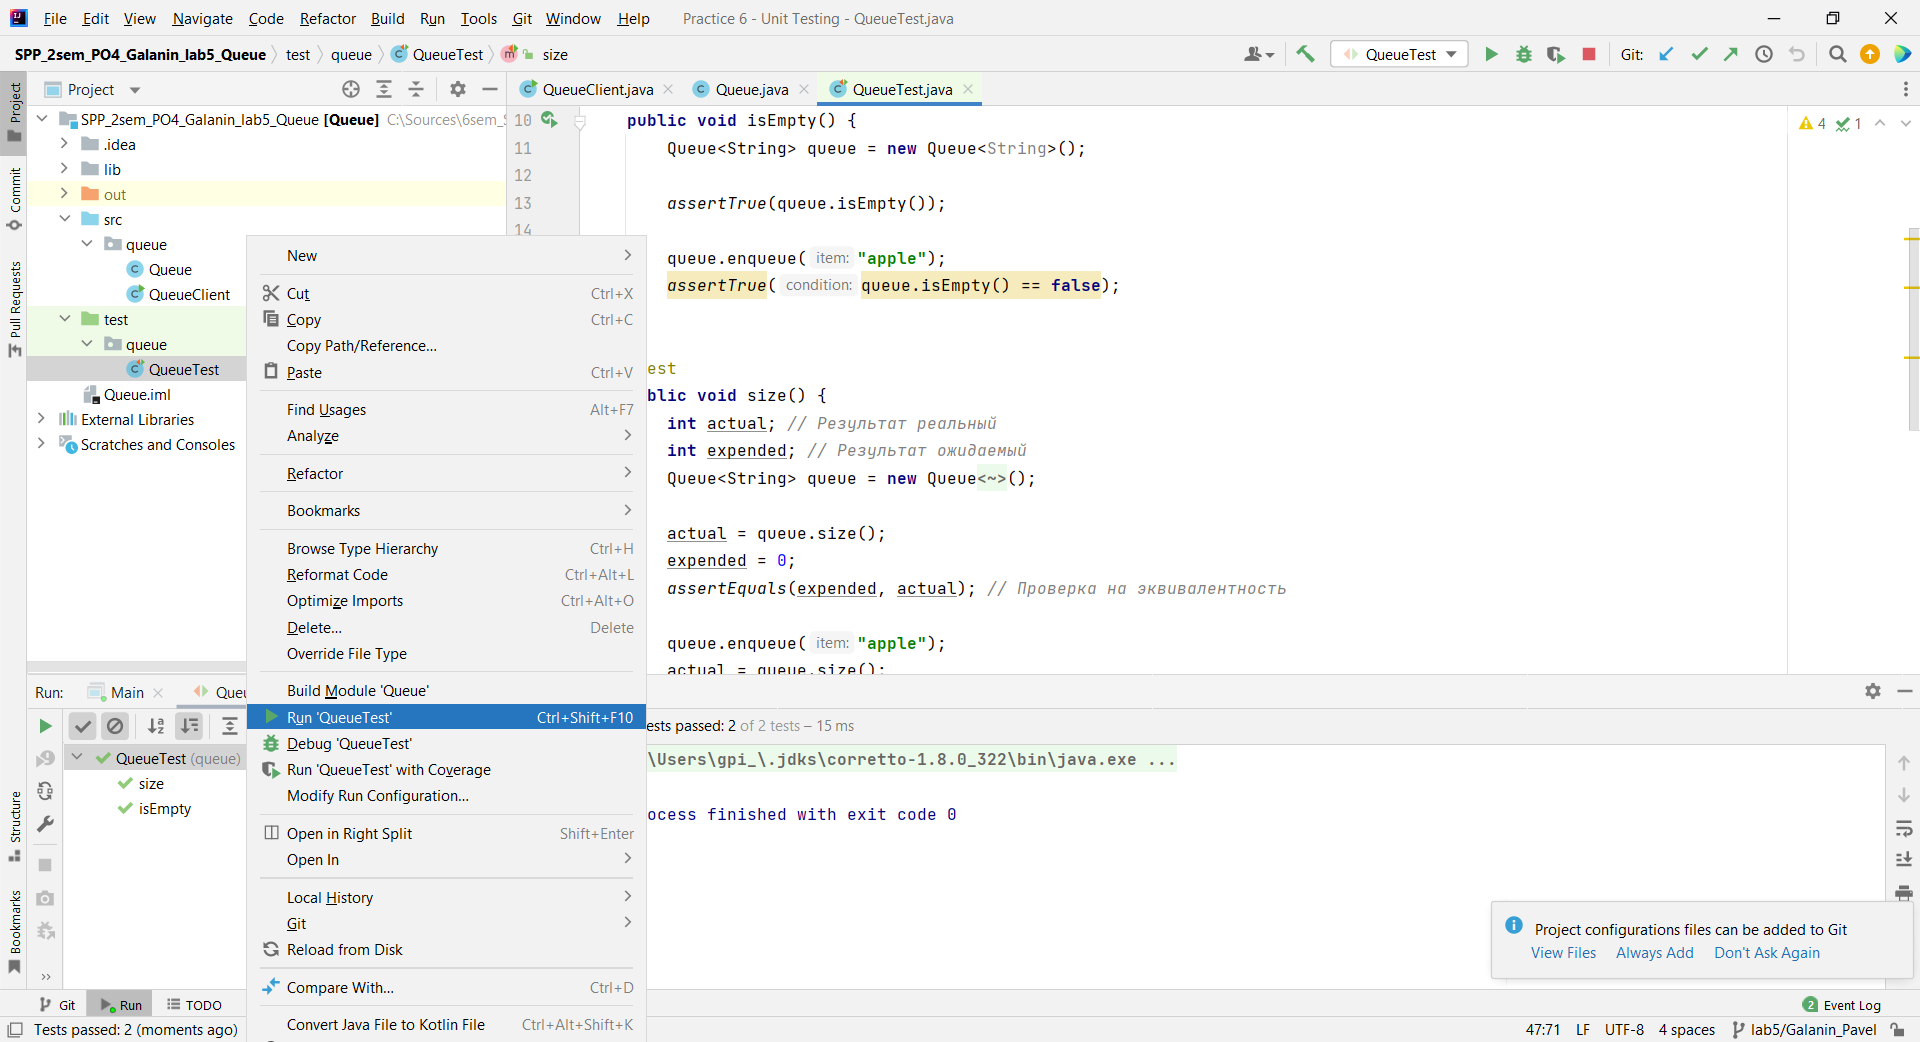
\includegraphics[width=16cm]
            {_assets/QueueTest.png}
        \caption{Скриншот пройденных тестов класса Queue}
    \end{figure}

%     \paragraph{} \textbf{Вывод}: создали отчёт, используя \LaTeX.

    % = = = = = = = =
    % \newpage
    % \addcontentsline{toc}{section}{Список использованных источников}
    % \section*{Список использованных источников}
    \paragraph{} \textbf{Список использованных источников}:
    \begin{enumerate}
        \item[1.] Как создать и запустить простой JUnit тест? Что такое JUnit и как работает юнит-тестирование в Java? - YouTube [Электронный ресурс]
        - Режим доступа: \url{https://www.youtube.com/watch?v=GQKDVSuqQlI}.
        Дата~доступа:~08.05.2022.
        \item[2.] Download and Install · junit-team/junit4 Wiki [Электронный ресурс]
        - Режим доступа: \url{https://github.com/junit-team/junit4/wiki/Download-and-Install}.
        Дата~доступа:~08.05.2022.
        \item[3.] Maven Central Repository Search [Электронный ресурс]
        - Режим доступа: \url{https://search.maven.org/search?q=g:junit%20AND%20a:junit}.
        Дата~доступа:~08.05.2022.
        \item[4.] junit - java.lang.NoClassDefFoundError: org/hamcrest/SelfDescribing in Intellij - Stack Overflow [Электронный ресурс]
        - Режим доступа: \url{https://stackoverflow.com/questions/17594483/java-lang-noclassdeffounderror-org-hamcrest-selfdescribing-in-intellij}.
        Дата~доступа:~08.05.2022.
        \item[5.] org.hamcrest : hamcrest-core : 1.3 - Maven Central Repository Search [Электронный ресурс]
        - Режим доступа: \url{https://search.maven.org/artifact/org.hamcrest/hamcrest-core/1.3/jar}.
        Дата~доступа:~08.05.2022.
    \end{enumerate}
    \newpage
\end{document}
